
%(BEGIN_QUESTION)
% Copyright 2012, Tony R. Kuphaldt, released under the Creative Commons Attribution License (v 1.0)
% This means you may do almost anything with this work of mine, so long as you give me proper credit

PT-58, PRC-58, and PV-58 comprise a gas pressure control system to monitor and regulate gas pressure in this oil/natural-gas separator vessel by venting excess natural gas to the flare.  During normal operation, there is just a little bit of gas flow vented to the flare.  Most of the gas exits the separator vessel through control valve FV-66:

$$\includegraphics[width=15.5cm]{i03538x01.eps}$$

Suppose one day the flow transmitter FT-66 fails with a high output signal (i.e. 20 mA) with the flow controller in automatic mode.  How will this affect gas pressure and liquid level control in this system, after enough time has passed for all variables to reach a steady-state condition again?  Assume the controllers are in automatic mode and have been properly tuned.  Explain your reasoning for the effects on gas pressure and liquid level, not just what happens to each.

\underbar{file i03538}
%(END_QUESTION)





%(BEGIN_ANSWER)

\noindent
5 points for each correctly-reasoned answer:

\vskip 10pt

Gas pressure will {\bf remain at setpoint} inside the separator vessel because PRC-58 is still actively sensing and controlling pressure by relieving excess gas to the flare.  

\vskip 10pt

Liquid level will also {\bf remain unchanged}, as LT-83 and LC-83 will continue to operate normally.  

\vskip 10pt

What will change is that more gas will be flared off, and no gas will flow to the gas treatment process because FV-66 will slam shut.


%(END_ANSWER)





%(BEGIN_NOTES)

{\bf This question is intended for exams only and not worksheets!}.

%(END_NOTES)


